
\documentclass[a4paper]{article}

\usepackage{inputenc}
\usepackage[british,UKenglish]{babel}
\usepackage{amsmath}
%\usepackage{titlesec}
\usepackage{color}
\usepackage{graphicx}
\usepackage{fancyref}
\usepackage{hyperref}
\usepackage{float}
\usepackage{scrextend}
\usepackage{setspace}
\usepackage{xargs}
\usepackage{multicol}
\usepackage{nameref}

\usepackage{sectsty}
\usepackage{multicol}
\usepackage{multirow}
\usepackage[procnames]{listings}
\usepackage{appendix}
\usepackage{listings}
\usepackage{booktabs} % 导入三线表需要的宏包
\usepackage{array}
\usepackage{indentfirst} 
\setlength{\parindent}{2em} %段落缩进

\newcommand\tab[1][1cm]{\hspace*{#1}}
\hypersetup{colorlinks=true, linkcolor=black}
\interfootnotelinepenalty=10000

\newcommand{\cleancode}[1]{\begin{addmargin}[3em]{3em}\texttt{\textcolor{cleanOrange}{#1}}\end{addmargin}}
\newcommand{\cleanstyle}[1]{\text{\textcolor{cleanOrange}{\texttt{#1}}}}


\usepackage[colorinlistoftodos,prependcaption,textsize=footnotesize]{todonotes}
\newcommandx{\commred}[2][1=]{\textcolor{Red}
{\todo[linecolor=red,backgroundcolor=red!25,bordercolor=red,#1]{#2}}}
\newcommandx{\commblue}[2][1=]{\textcolor{Blue}
{\todo[linecolor=blue,backgroundcolor=blue!25,bordercolor=blue,#1]{#2}}}
\newcommandx{\commgreen}[2][1=]{\textcolor{OliveGreen}{\todo[linecolor=OliveGreen,backgroundcolor=OliveGreen!25,bordercolor=OliveGreen,#1]{#2}}}
\newcommandx{\commpurp}[2][1=]{\textcolor{Plum}{\todo[linecolor=Plum,backgroundcolor=Plum!25,bordercolor=Plum,#1]{#2}}}

\def\code#1{{\tt #1}}

\def\note#1{\noindent{\bf [Note: #1]}}

\makeatletter
%% The "\@seccntformat" command is an auxiliary command
%% (see pp. 26f. of 'The LaTeX Companion,' 2nd. ed.)
\def\@seccntformat#1{\@ifundefined{#1@cntformat}%
   {\csname the#1\endcsname\quad}  % default
   {\csname #1@cntformat\endcsname}% enable individual control
}
\let\oldappendix\appendix %% save current definition of \appendix
\renewcommand\appendix{%
    \oldappendix
    \newcommand{\section@cntformat}{\appendixname~\thesection\quad}
}
\makeatother




\lstset{frame=, basicstyle={\footnotesize\ttfamily}}



\graphicspath{ {images/} }
\usepackage{ctex}



\usepackage[square,numbers]{natbib}
\bibliographystyle{unsrt}


\begin{document}
\renewcommand{\contentsname}{目\ 录}
\renewcommand{\appendixname}{附录}
\renewcommand{\appendixpagename}{附录}
\renewcommand{\refname}{参考文献}

\renewcommand{\tablename}{表}
\renewcommand{\today}{\number\year 年 \number\month 月 \number\day 日}

\title{{\Huge 可视语言与信息可视化{\large\linebreak\\}}{\Large 团队ID: 20\linebreak}
{\Large  \linebreak\linebreak}}
\author{ \large
  刘京宗 3019213043
  \\\\
  杨朝涵 3020244160
  \\\\
  张雪雅 3020244317
  \\\\\\
  天津大学,智能与计算学部}
\date{\today}
\maketitle
\newpage

\begin{center}
  \tableofcontents\label{c}
\end{center}
\newpage


\begin{center}
  {\Large\bf{摘\ 要\\}}

  % 大作业要求大家按照论文短文的格式进行书写,参考文献~\cite{bayrak2020pragma, govyadinov2019graph}。



\end{center}

\newpage



\section{引言}
\label{overview}
\begin{figure}[htbp]
  \centering
  
\includegraphics[width=1\textwidth]{images/MC3.jpg}
  \caption{背景}\label{fig:MC3}
  \vspace{\baselineskip}
\end{figure}
2014年1月23日,阿比拉发生了多起事件。系统已要求您根据发生的有限信息进行回顾性分析。您的目标是确定风险以及如何更有效地缓解风险。

您可以访问包含两个主要来源的单个数据流:

由自动筛选器识别为与正在进行的事件潜在相关的微博记录

阿比拉,克罗诺斯岛地方警察和消防部门的紧急调度文字记录。

根据这些数据,您可以评估公众不断变化的风险水平并提出建议的措施吗?

您还可以访问阿比拉地图和背景文件。 (注意:这些是“迷你挑战1”和“迷你挑战2”中提供的相同材料)

使用视觉分析来分析可用数据并制定对要提供的问题的响应。此外,准备一段视频,展示您如何使用视觉分析来解决这一难题。

\section{相关工作}

% 调研相关论文发表,搜索CNKI或者Google scholar 等学术引擎,了解该领域研究现状。参考文献格式为~\cite{bayrak2020pragma,chen2018embed}。
作为一门问题和目标主要来自于现实世界的学科,数据可视化在很多领域获得了研究、应用和长足进
步,在从研究范围(广度)、研究精细化(深度)不断拓展学科边界的过程中,逐渐收敛成为若干热点领域。本
文以数据特征来划分,介绍其中的3类技术。
\subsection{时间序列数据可视化}
时间序列可视化随着时间的发展采集信息数据,运用
可视化技术手段进行呈现,呈现出的可视化方式主要有3
种。一是线形图,通过最开始的点展示不同时间段
信息数据变化,在可视化过程中信息数据呈现较多时间维度,根据不同维度建立相应图标进行排列,观察数
据的变化\textsuperscript{~\cite{chen2018embed}};二是堆积图,这类图主要对所有时间序列进行叠加,出现负数时,堆积图无法处理所有的
时间序列,极大程度降低了可视化的呈现效果;三是地平线图,随着时间变化清楚地观察到信息数
据的变化率,颜色的深浅表示正向、负向的变动效果\textsuperscript{~\cite{ali2019timecluster,suh2019persistent}}。
\subsection{网络数据可视化}
网络数据可视化技术手段核心是自动布局算法,将信息数据通过自动布局、计算,绘制成网状结构的图
形。应用较广泛的有3类。力导向布局:借助力的概念,连接受力节点绘制网状图,由于互斥力的
存在,可以减少节点间的重叠,适用于描述事物之间的关系,例如计算机网络关系、社交网络关系等各类关系
网络情景\textsuperscript{~\cite{韩刘2020多元异构网络复杂多维数据可视化方法,王悦2020可视化指导下的图像领域深度学习模型优化方案设计}}。圆形布局:将所有节点自定义排序,按照顺序在圆形上排列出来,快速分析出结
果,受限于屏幕大小,节点数量较多时,圆形半径越来越大,难以直观显示全部节点,适用于查找较多关联关
系的节点场景,例如在圆形布局图中可明显分辨出哪些节点关联关系较多。网格布局:采用网格
设计方式绘制网格状信息数据网状图,适用于分层网络,利于观察整体层次
\textsuperscript{~\cite{田丰2019自然人机交互新进展专题前言}}。
\subsection{层次信息数据可视化}
层次结构常被用来描述具有明显层次结构的对象,包括图书馆标签、计算机层次系统或者面向对象程序
类之间的继承关系等\textsuperscript{~\cite{田宇荃2020海绵城市建设前后的可视化效果分析,陶芳2019网络舆论数据可视化技术研究}}。层次信息数据可视化用到的方法主要包括节点连接、空间填充、混合方法等。
节点连接主要绘制不同形状节点表示信息数据内容,节点之间连线表示数据之间的关系。此
类层次代表技术有空间树、圆锥树等。
空间填充主要运用包围框表示层次结构信息数据,上层节点与下层节点之间包围关系表示信息数据间
的结构关系\textsuperscript{~\cite{张甜甜2020一种基于数独分组的拉丁超立方试验设计方法}}。此类层次代表技术有树图、信息立方体等。
混合方法结合多种可视化技术优点,使认知行为更加高效\textsuperscript{~\cite{zhang2021interactive}}。此类方法代表技术有弹性层次层次网等。
\section{问题描述和需求分析}
\label{Data and Task Abstraction}
使用视觉分析来表征数据集中不同类型的内容。什么是有意义的事件报告与典型的垃圾邮件或垃圾邮件区别开来?请将答案限制为8张图片和500个单词。

使用可视化分析来表示和评估在晚上的过程中对公众的风险程度如何演变。考虑这种情况的潜在后果以及可能受到影响的人数。请将答案限制为10张图片和1000字。

如果您能够将一组急救人员发送到任何地方,它将在哪里?提供您的理由。如果您必须实时而不是回顾性地响应事件,那么您的响应会有什么不同?请将答案限制为8张图片和500个单词。

\section{解决方案}
\subsection{任务一}
(1)借助Python处理数据,提取message中的tag,并且统计每个tag出现的次数,据此绘制词云。

(2)借助Python处理数据,对message进行分类,借助散点图和柱状图表征数据集中不同类型的内容。

(3)使用tf-idf算法,对不同类型的message提取关键词,并且用TreeMap展示。

(4)统计不同类型的message的作者信息,同样用TreeMap进行展示。
\subsection{任务二}
\subsection{任务三}
(1)提取不同时间段关键词,依据此关键词得出此时段事件,依据事件绘制事件流图。

(2)借助Python处理数据,筛选出所有含有latitude和longitude的数据,再筛选出与特定事件即dancing dolphin fire有关的数据,据此绘制出latitude-longitude坐标图。

(3)借助Python处理数据,筛选出所有含有location的数据,再筛选出含有关键字fire的数据,据此绘制词云。

(4)提取指定时间段关键词,选择出现次数多且有意义的关键词数据,据此绘制关键词饼图。

\section{实验结果和案例分析}\label{sub:ptxeva}
\subsection{任务一}

统计不同tag在message中出现的次数,如图~\ref{fig:1-tags}~所示。

\begin{figure}[H]
  \centering
  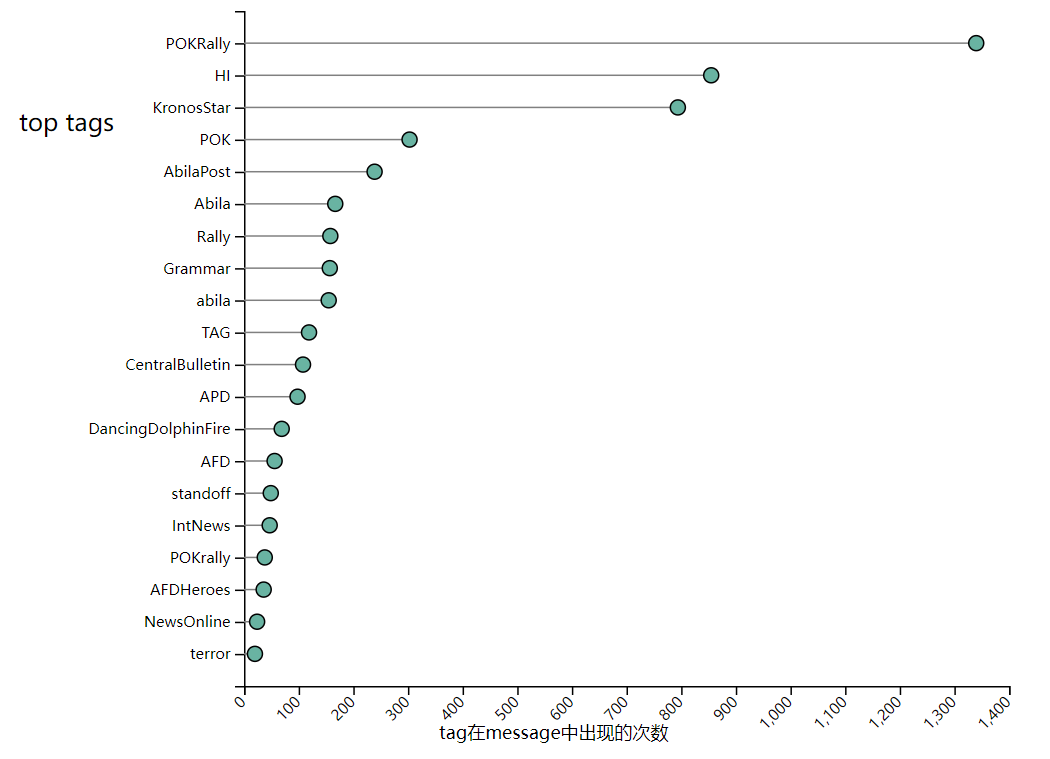
\includegraphics[width=0.9\textwidth]{images/1-tags.png}
  \caption{不同tag在message中出现的次数}\label{fig:1-tags}
  \vspace{\baselineskip}
\end{figure}
\begin{figure}[H]
  \centering
  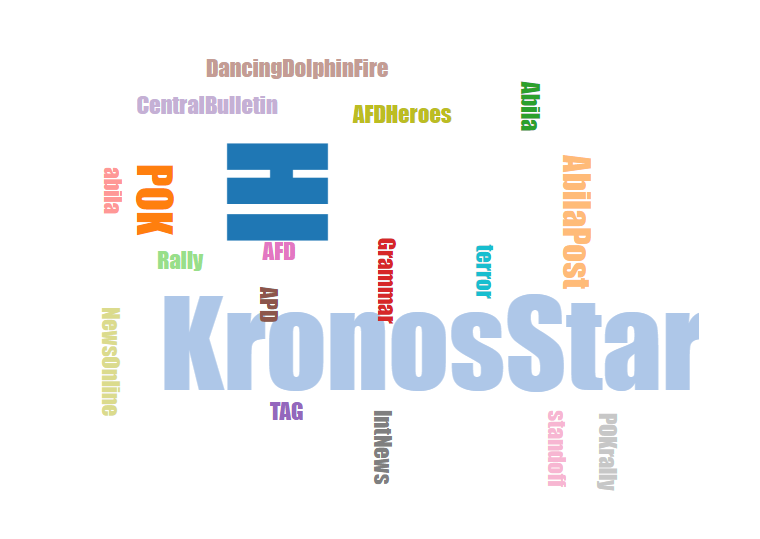
\includegraphics[width=0.8\textwidth]{images/1-wordcloud.png}
  \caption{tag词云}\label{fig:1-wordcloud}
  \vspace{\baselineskip}
\end{figure}
通过这些tag,我们可以对message的主题有一个把握,并且词云的形象化展示,让我们对数据有了更直观的认识。

借助Python处理数据,对message进行分类,具体如表~\ref{tab:table1}~所示。
\begin{table}[H]
  \caption{不同类别的message分类说明}\label{tab:table1}
  \vspace{0.5em}\centering
  %设置表格的宽度不超过页面长度
  \begin{tabular}{|p{2.2cm}<{\raggedright}|p{8.5cm}<{\raggedright}|}
    \toprule[1.5pt]
    种类          & 说明                                                                                                                                      \\                                                                                                                               \\
    \midrule[1pt]
    unrelated     & 与报道完全无关的消息。主要由用户@KronosQuoth和@Clevvah4Evah发出。二人的消息主要是一些“心灵鸡汤”、励志格言,与报道内容完全无关,共1418条。 \\ \hline
    advertisement & 广告。其内容中往往包含了网页链接,如“I recommend this site \#abila dates.kronos/clickhere” 借助正则表达式'.*\..*/'进行筛选,共227条。     \\ \hline
    chatter       & 闲聊。这部分内容主要为用户的闲聊,主要特征为通常以“RT @”开头,共1006条                                                                    \\ \hline
    report        & 报道。主要为当地媒体对新闻的报导,如关于火灾,枪击的报道。主要由@AbilaPost, @megaMan等用户发送,共424条。                                 \\ \hline
    others        & 其他。不能被以上四类所典型概括的消息,统一归为其他,共988条。                                                                             \\ \hline
    \bottomrule[1.5pt]
  \end{tabular}
  \vspace{\baselineskip}
\end{table}
在对message进行分类后,我们采用散点图和柱状图表征数据集中不同类型message的内容.
\begin{figure}[H]
  \centering
  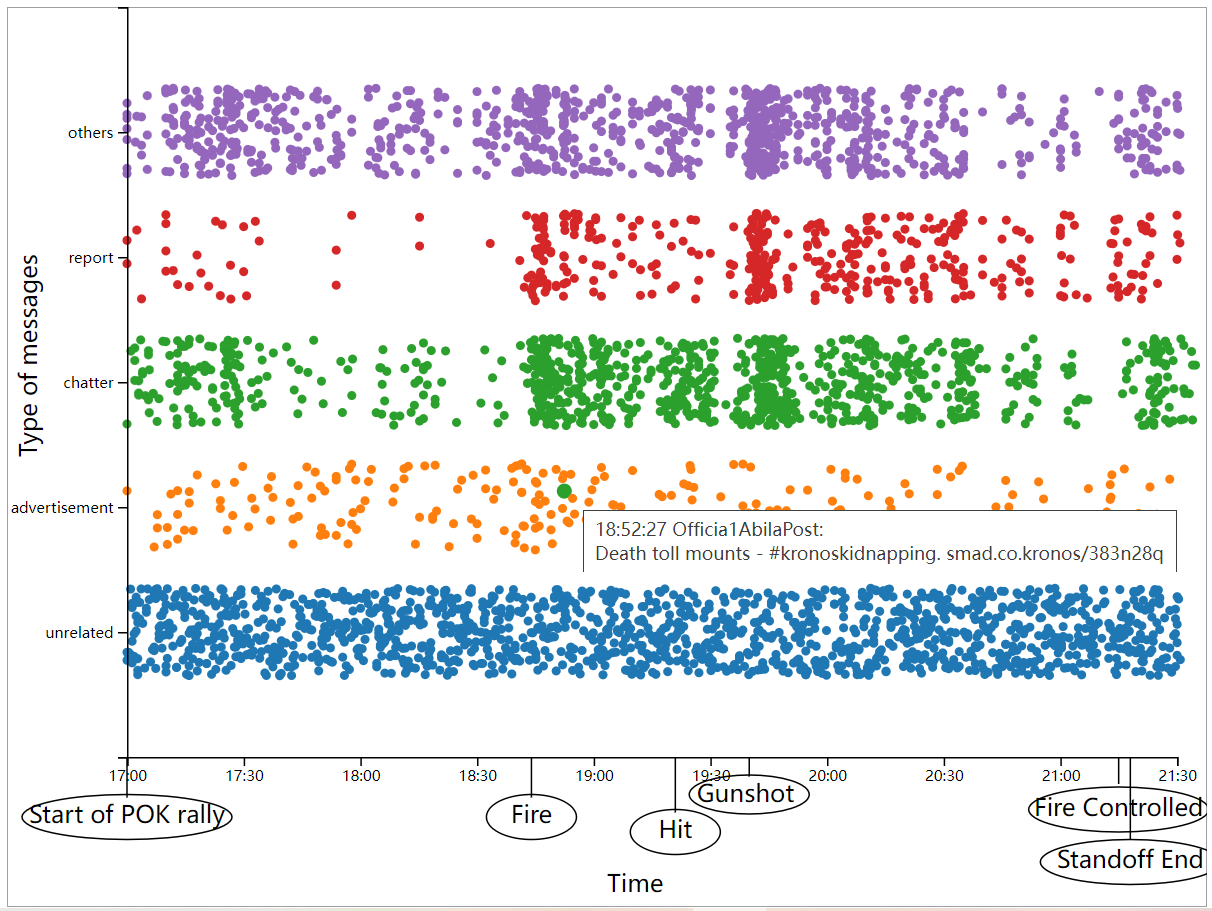
\includegraphics[width=0.95\textwidth]{images/1-scatter-2.png}
  \caption{散点图}\label{fig:1-scatter}
  \vspace{\baselineskip}
\end{figure}
\begin{figure}[H]
  \centering
  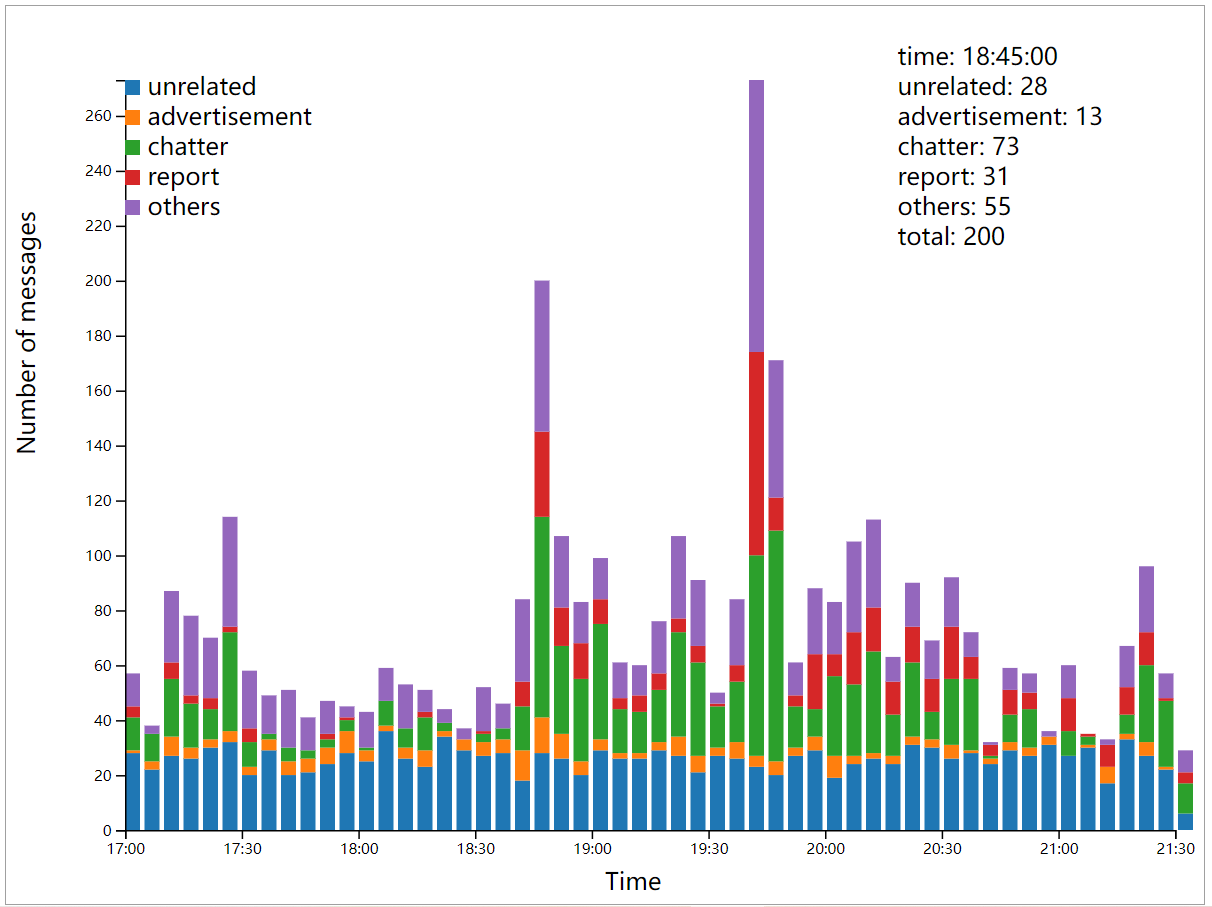
\includegraphics[width=1\textwidth]{images/1-bars-2.png}
  \caption{柱状图}\label{fig:1-bar}
  \vspace{\baselineskip}
\end{figure}
通过散点图和柱状图,我们可以对不同类型的message随时间的变化有一个直观的认识。且我们能直观感受到有重大事件(如图~\ref{fig:1-scatter}~横轴所示)发生时,
chatter和report类型的消息数量会有一个明显增加。
且我们为这两幅图增加了一定的交互性,当鼠标悬停在散点图中的点上时,会
有颜色变化,同时显示出该点对应的message信息,包括时间与作者信息。当
鼠标悬停在柱状图中的柱子上时,会显示出该柱子对应的时间段以及该时间段内
的各种message的数量。

之后,我们使用tf-idf算法对message进行关键字提取,使用TreeMap对这些关键字进行可视化,
通过关键词简洁明了地展示不同类别的message的内容。类似的,我们统计了不同类别的message的
作者信息。同样选择使用TreeMap对这些信息进行可视化。具体如~\ref{fig:1-keyword}~和~\ref{fig:1-author}~所示。
\begin{figure}[H]
  \centering
  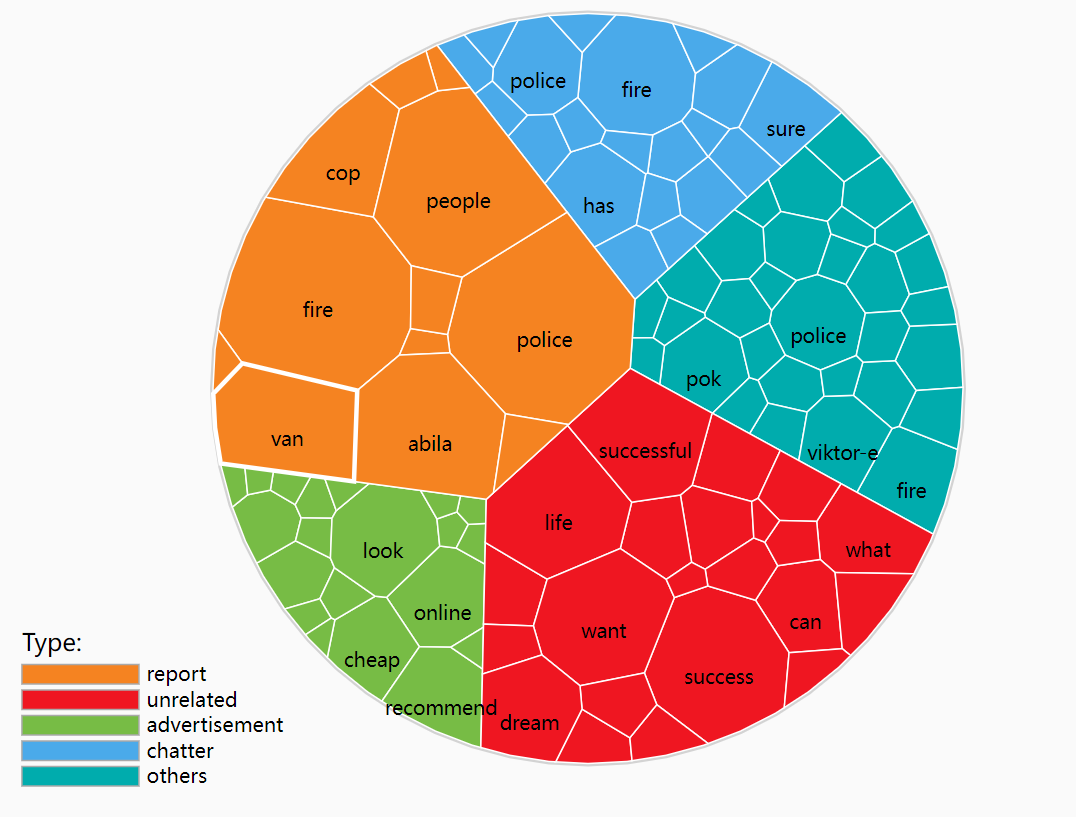
\includegraphics[width=0.95\textwidth]{images/1-keyword.png}
  \caption{关键词TreeMap可视化}\label{fig:1-keyword}
  \vspace{\baselineskip}
\end{figure}
\begin{figure}[H]
  \centering
  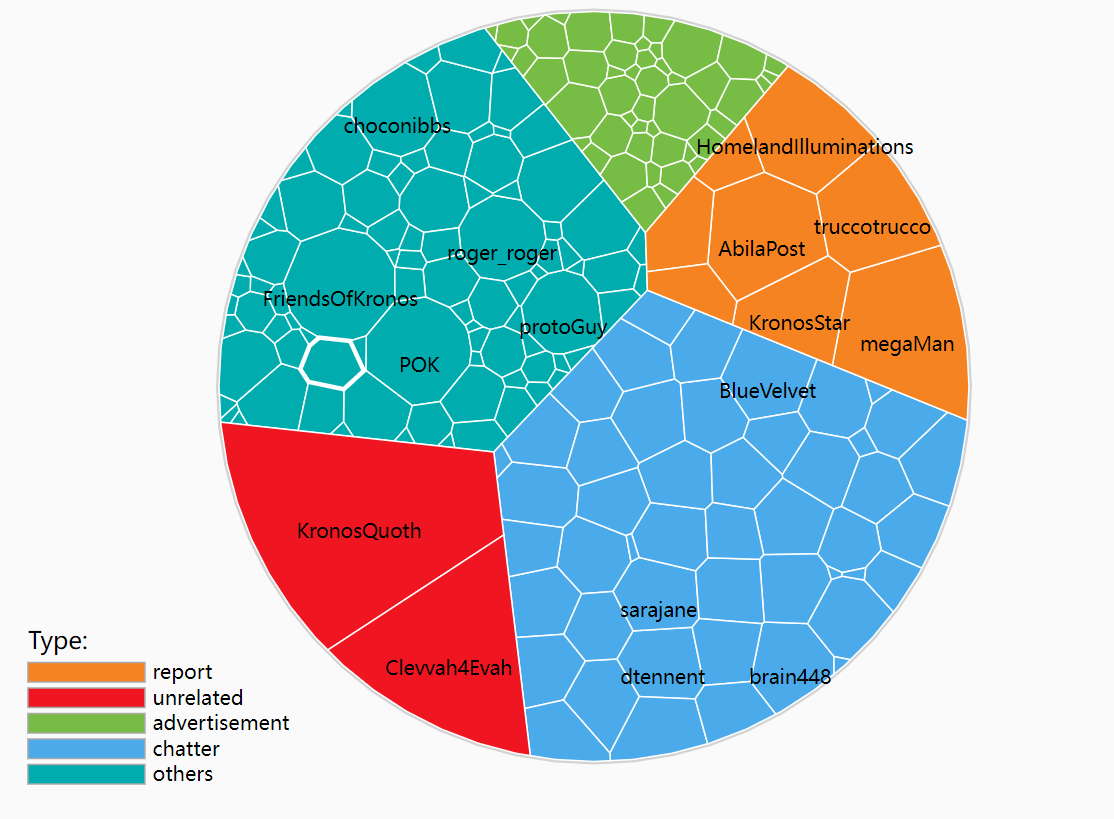
\includegraphics[width=0.95\textwidth]{images/1-author.png}
  \caption{作者TreeMap可视化}\label{fig:1-author}
  \vspace{\baselineskip}
\end{figure}
在上述两幅图中,我们选择展示面积占比较大的关键词和作者,以便于我们对数据集中的内容有一个直观的认识。
对于占比较小的关键词和作者,只有鼠标悬浮在其上时才会显示出其具体信息。

\subsection{任务二}
\subsection{任务三}
Question1:如果您能够将一组急救人员发送到任何地方,它将在哪里?

Ansewer1:急救人员将被派往火灾发生地附近,其经度为36.059,纬度为24.894,位置为N. Achilleos St / N. Madeg St。

\begin{figure}[H]
  \centering
  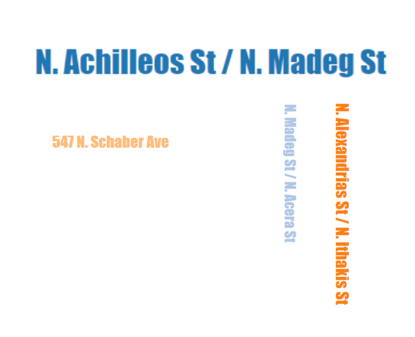
\includegraphics[width=0.9\textwidth]{images/3-2.png}
  \caption{location}\label{fig:3-2}
  \vspace{\baselineskip}
\end{figure}

Cause1:依据得出的各个时间段的关键词信息,可以得出事件流如图所示。

可以直观看出火灾在18:40发生;19:00时火势失控,同时开始扩大疏散区域;后续火势持续失控,在20:30时顶层发生坍塌;21:30时发生爆炸且有人员受伤。在火灾事件中,自火灾发生,火势近三小时内一直未得良好控制,属于高风险度事件;同时,发生了坍塌和爆炸此类重大风险事件,爆炸影响范围超出人群疏散范围,严重危害到群众的生命财产安全。

反观发生在19:40的警匪对峙事件为高风险度事件,起因为19:20发生的肇事逃逸,被撞人员并未受伤。19:40时发生枪战,货车司机绑持人质,一名警员在枪战中受伤倒地,评估为高风险度事件;19:55救护车救治受伤警员,大约15min后发布报道称警员处于危险但稳定的状态下;后续,对峙持续进行,警察发布公告远离此区域并保持静止;最终,在21:15,货车司机放弃抵抗,人质获救。对峙事件和平结束,无消息表明除警员外有其他人受伤,受伤警员已被救治且无生命危险。

综上,警匪对峙事件与火灾事件相较,影响范围小,受伤人群少,风险系数较低。在枪战事件中,货车司机向警察开枪,除人质外并未袭击普通群众,同时,普通群众有能力寻找掩蔽体以保护自身安全,最后,可以确定除警员外无人员受伤;而在火灾,尤其是后续的爆炸事件中,群众无法估计或错误估计其影响范围,在爆炸发生时无法实施自救,同时已明确有人员受伤,在建筑内可能也存在未被解救人员,更为危险,更需要急救人员在场。所以,回顾事件,急救人员应被派往火灾发生地附近,应及时救治在火灾、坍塌、爆炸事件中受伤人群。

Question2:如果您必须实时而不是回顾性地响应事件,那么您的响应会有什么不同?

Answer2:若实时性响应事件,急救人员将被派往警匪枪战对峙事件发生地附近,其经度为36.059,纬度为24.856。

Cause2:考虑到火灾事件18:40时发生,19:30时警察扩大人群疏散范围,提取了自19:30至19:32时的信息关键字数据;考虑到对峙事件19:40左右发生,提取了自19:41至19:43时的信息关键字数据。选取两份数据中出现次数最多的且有意义的关键字,可视化其比例分布饼图,如图所示。

\section{总结}
刘京宗:

在本次实验中,我主要负责任务一的完成。对于我这部分内容来说,在进行可视化之前,需要
对数据集进行预处理,这部分工作花费了我较多的时间。但这部分工作一方面让我熟悉了Python的一些
语法和相关库的使用,也是后续可视化工作的基础。在进行可视化工作时,我还是对
D3.js的接口不够熟悉,这也是我在本次实验中遇到的最大的困难。但在查阅相关资料后,
我对D3.js有了一定的了解,也完成了本次实验的任务一。最后通过撰写文档,
我对Latex的使用也有了一定的了解。总的来说,本次实验让我收益匪浅。

张雪雅:

在本次大作业中,我主要负责任务三的部分。
在此部分,我认为最重要的是在对数据分析后进行的思考,也耗时最久。
因为本任务为开放性问题,要首先通过数据分析确定出发角度,沿此思路完成后续对数据信息的可视化。
在数据分析阶段,沿用了任务一中的思路,利用python进行数据提取,因有良好基础,这部分并不复杂;
比较困难的是对有用数据进行筛选,但通过资料的查阅也得到良好解决。
在数据可视化阶段,这是本次大作业的重中之重,在数据的基础上考虑可视化样式,因刚接触d3不久,对此方式可视化数据不是非常熟悉,在这阶段耗时较久,通过回顾理清html和js语言,最终完成了本次绘制。
在报告撰写阶段,因在之前小学期阶段,已使用过latex撰写报告,这部分并不困难,在完成报告的过程中,再次梳理任务完成思路,回顾历程。
总之,本次大作业从方方面面都带给我很大的收获!
%新加一页
\newpage
\bibliography{ref}
\end{document}

